\documentclass[10pt]{article}
\usepackage[polish]{babel}
\usepackage[utf8]{inputenc}
\usepackage[T1]{fontenc}
\usepackage{amsmath}
\usepackage{amsfonts}
\usepackage{amssymb}
\usepackage[version=4]{mhchem}
\usepackage{stmaryrd}
\usepackage{graphicx}
\usepackage[export]{adjustbox}
\graphicspath{ {./images/} }

\title{GIMNAZJUM }

\author{}
\date{}


\begin{document}
\maketitle
\begin{enumerate}
  \item Rozwiąż w liczbach całkowitych równanie
\end{enumerate}

\[
x(x+1)+(x+1)(x+2)+\cdots+(x+9)(x+10)=2016 x+2015
\]

\begin{enumerate}
  \setcounter{enumi}{1}
  \item Dany jest 2016-kąt foremny. Na ile sposobów można wybrać cztery spośród jego wierzchołków tak, aby były one wierzchołkami kwadratu?
  \item Czy długości boków, na które dzielą się dwie przecinające się cięciwy okręgu mogą wyrażać się czterema kolejnymi liczbami naturalnymi?\\
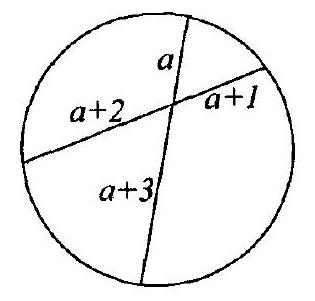
\includegraphics[max width=\textwidth, center]{2024_11_21_93cdd7e5dcdd6a9af56eg-1}
\end{enumerate}

\section*{LICEUM}
\begin{enumerate}
  \item Na jednokierunkowej trasie znajduje się tunel o przekroju półelipsy. Szerokość jezdni wynosi 12 m , a najwyższy punkt tunelu znajduje się na wysokości 5 m nad jezdnią. Jaka może być maksymalnie wysokość kontenera szerokości 4 m , który można przewieźć tą trasą na platformie wysokości 1 m ?
  \item Ile rozwiązań w przedziale \(\langle 0, \pi\rangle\) ma równanie \(\sin x \cdot \cos x=\sin 40^{\circ}\) ?
  \item Rozwiązaniami równania \(23 x^{3}-15 x^{2}-x+1=0\) są liczby \(a, b, c\). lle jest równa liczba \((a+1)(b+1)(c+1)\) ?
\end{enumerate}

\end{document}